\documentclass[10pt,letterpaper]{article}

\usepackage{graphicx}
\usepackage[parfill]{parskip}
\usepackage{fullpage}
\usepackage{amsmath}
\usepackage{amssymb}
%\usepackage{amsthm}

%\usepackage{wrapfig}
\usepackage{caption}
\captionsetup{format=plain,labelformat=empty}
\usepackage{framed}
\title{Super Fast Galaxy: UGC-12591!}
%\author{EmD}
%\date{}


\usepackage{fancyhdr}
\makeatletter
\renewcommand\footnoterule{%
  \kern23\p@
  \hrule\@width\linewidth
  \kern2.6\p@}
\makeatother 

\pagestyle{fancy}
\usepackage{lastpage}
\setlength{\headheight}{15pt}
\setlength{\headsep}{0.4in}
\fancyhead{}
\chead{\textbf{Super Fast Galaxy: UGC-12591!} }
\lhead{EmD}
\rhead{\today }
\fancyfoot{}
\setlength{\footskip}{17pt}
%\renewcommand{\footrulewidth}{0.4pt}
%\cfoot{Page \thepage/\pageref{LastPage}}
%\lfoot{UGC-12591}
%\rfoot{Posts}


\usepackage{url}
\usepackage{hyperref}
\hypersetup{
    colorlinks=true,
    linkcolor=blue,
    anchorcolor=black,
    citecolor=green,
    linktocpage=true,
    filecolor=magenta,      
    urlcolor=cyan,
    pdftitle={UGC-12591},
    pdfauthor={EmD},
pdfpagemode=FullScreen,
}


\begin{document}
%\maketitle

\begin{figure}[!ht]
\begin{framed}
\begin{center}
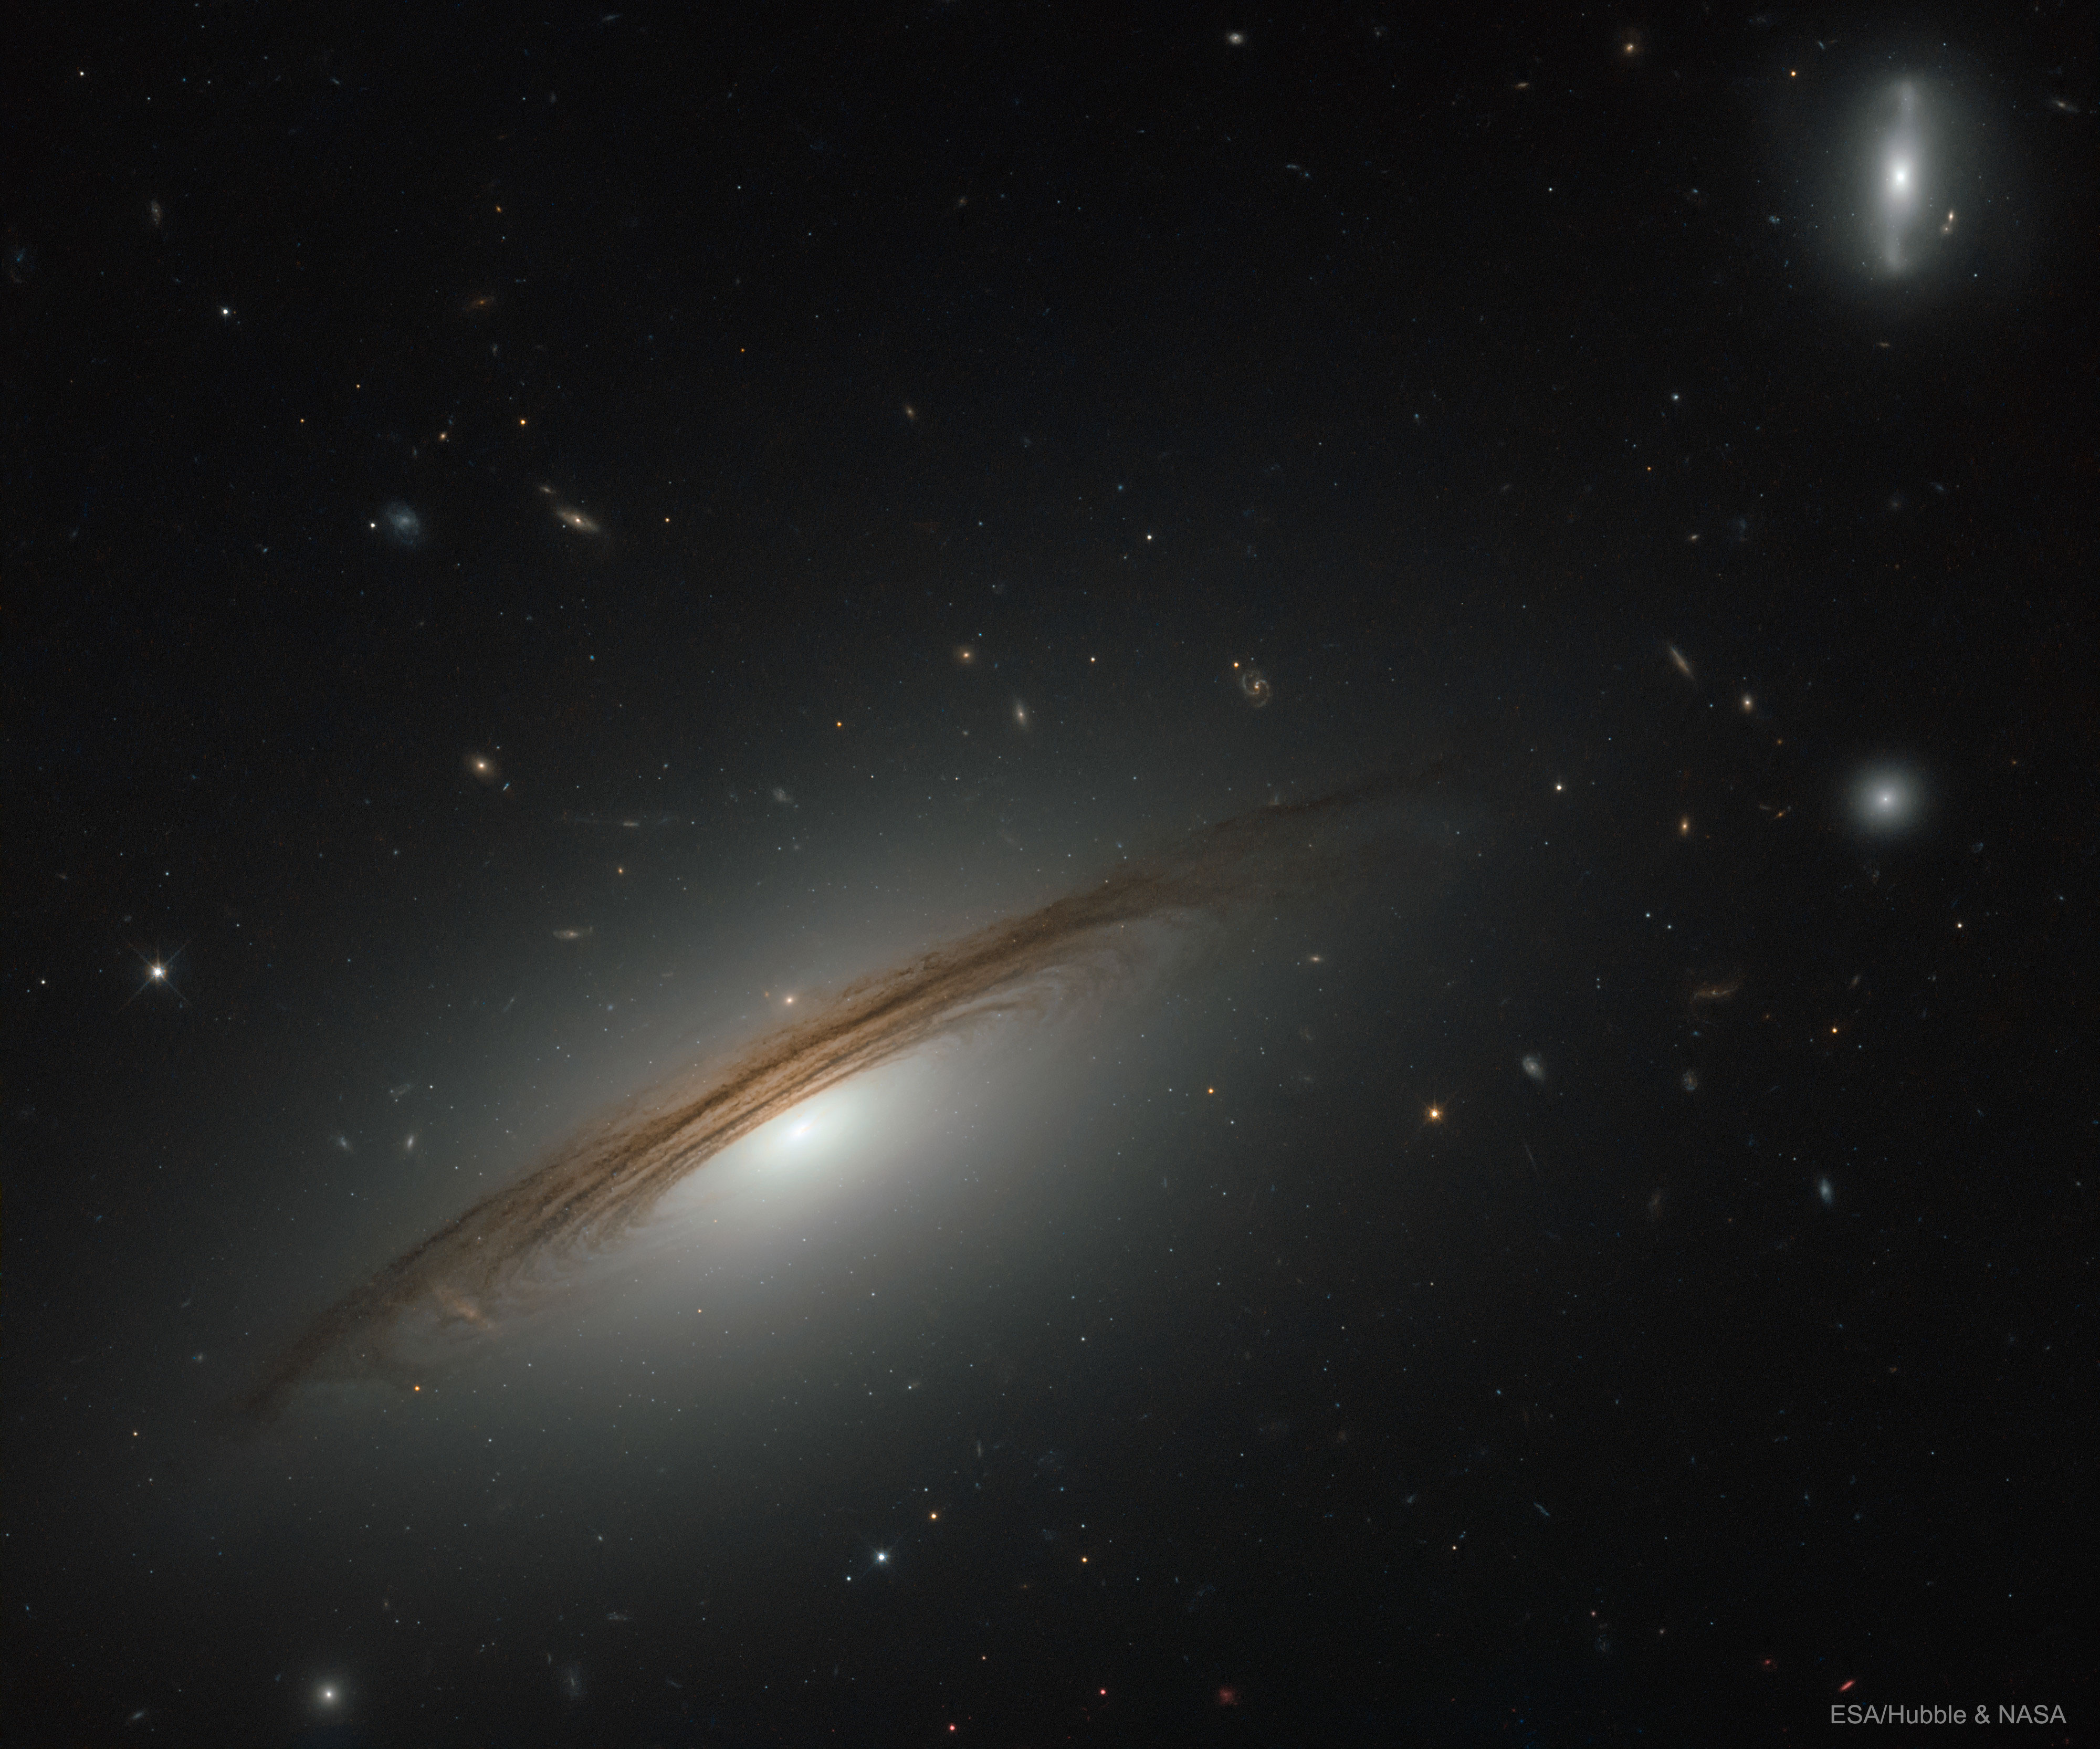
\includegraphics[width=0.75\textwidth]{../Images/UGC125991.jpg} 
\caption{This is galaxy UGC-12591!}
\end{center}
\end{framed}
\end{figure}




\section*{What's so cool about this galaxy?}

UGC-12591\footnote{kind of just rolls off the tongue doesn't it} is the fastest spinning galaxy we've found yet!

\textbf{Well just how fast are we talking here?}

UGC-12591 galaxy is spinning at a rate of about $480 km/sec$!

\textbf{What does that even mean?}

That is a great question! 

It means that UGC-12591 is spinning nearly twice as fast as our own Milky Way galaxy, which spins at around $270 km/sec$ or $168 mi/sec$. 

\textbf{Wait, if it spins so fast how come it doesn't tear itself apart? Why is it still sitting (spinning) there all in one piece?}

Another great question!

To answer this we need to ask, \textbf{what is rotation? Or what does it mean to rotate.}


\section*{Rotating and Revolving}

In astronomy a \textbf{rotation} usually refers to an object moving around an axis, a \textbf{revolution} in this field means that you are orbiting something external to yourself. \textit{The Earth revolves around our sun, and the Earth rotates about it's axis.}

When you stand up and spin you are \textit{rotating} around your own center of gravity. When you ride a Ferris wheel, you are \textit{revolving} around the center of the Ferris wheel. 

When it comes to galaxies and their components pinpointing what is revolving or rotating can be tricky but all these spinning movements still require enormous amounts of energy.

\section*{Spinning Takes Energy}

The Earth revolves around the sun in the same direction every time counterclockwise\footnote{anticlockwise}, it really does not want to go clockwise it wants to move in the same direction all the time. This resistance to a change in motion is what we call \textbf{mass}, it would take a hell of a shit ton of energy for the Earth to suddenly go clockwise around the sun\footnote{This would be a really, really bad thing, you probably wouldn't make it and neither would your dog.}. So from this perspective maybe we can see there is something going on between movement and energy, and between energy and mass\footnote{Likewise movement and mass etc.}, but how can we explore that relationship informally?


Luckily, there is a super famous equation which can tell us all kinds of things about the relationship between energy and mass:

\[e=mc^{2}\]

\textbf{What does that whole mess even mean and what the hell does it have to do with rotating?\footnote{I didn't ask for a low level diagnostic on astrophysics when I looked at the pretty picture.}}

Well we can interpret Einstein's famous equation to  mean \textit{energy is mass times the speed of light squared\footnote{roughly this is a huge over-simplification}}.

Remember that when we look at a galaxy we are looking at the light it produces, so to understand this equation we can momentarily ignore the speed of light and think about our question: \textbf{what does it mean to rotate?}

More or less, to rotate means to use energy by spinning around something. We've learned that spinning takes energy, and that mass is the resistance an object has to changing it's direction of movement.

Einstein's equation tells us that energy and mass are more or less interchangeable. 

\[Mass = Energy \\ Energy = Mass \footnote{times a very huge constant squared. We say that energy is directly proportional to mass times by a constant which even squared is still just a constant.} \]

So if something spins faster than something else and they are both being multiplied by the \textit{same} constant\footnote{the speed of light}, then the thing that is spinning faster has a mass that is as large (massive) as the energy it uses to do all that spinning. 

This answers our question:
\textbf{How come IGC-12591 doesn't rip itself apart when it spins?} 

The answer is because \textit{it has twice about twice as much mass as our own galaxy.}

Remember, we learned that UGC-12591 spins about twice as fast as our galaxy, so it makes sense that it has a mass nearly twice as large as our galaxy.

\section*{How Far Away is UGC-12591?}

\textbf{How old is the light we see from UGC-12591? Or, how far away is it?}

Well UGC-12591 is roughly 400 million light years from Earth.

The Milky Way galaxy is only about 100,000 light years across which is pretty tiny compared to 400 million light years. 

To make sense of just how big that is, think about some smaller more familiar spinning things. 

The Milky Way galaxy is around 100,000 light years in diameter.


Our solar system has a radius of about 1-3 light years, or 2-6 light years in diameter\footnote{it's not a circle so it depends where you measure across}; it is about $0.0032\%$ the size of the Milky Way.

Alternatively, if we shrank the entire Milky Way to the size of the United States, then our solar system would be about the size of an American penny. 

The average distance between the Earth and the Sun is around 150 million kilometers, (or 93 million miles); this distance is called an \textbf{Astronomical Unit} (AU). 

Light coming from our Sun takes about 8 minutes for us to see it on Earth, and the speed light travels is always the same no matter which source it is coming from (it's constant) which is $299,792 km/sec$ (or $186,287 miles/sec$). 

\begin{figure}[!ht]
\begin{framed}
\begin{center}
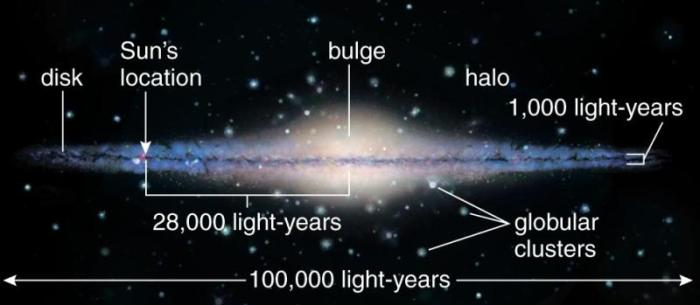
\includegraphics[width=0.75\textwidth]{../Images/diameter-milkyway.jpg} 
\caption{Diameter of the Milky Way Galaxy}
\end{center}
\end{framed}
\end{figure}

The light from UGC-12591 we are just now seeing here on Earth left that galaxy around 400 million years ago, which on Earth is around the time the first trees were developing (a really, really long time ago).

For more information about UGC-12591 visit \href{https://www.spacetelescope.org/images/potw1709a/}{Spacetelescope}
or
\href{http://www.space.com/35955-massive-hybrid-galaxy-hubble-telescope-photo.html}{Hubble Telescope}

\pagebreak

\begin{figure}[!ht]
\begin{framed}
\begin{center}
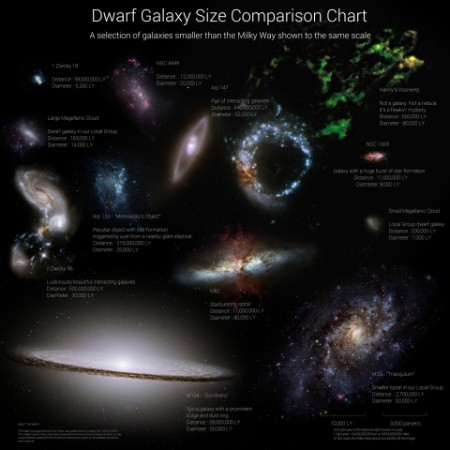
\includegraphics[width=0.75\textwidth]{../Images/comparegalaxies.jpg} 
\caption{Comparison of Dwarf Galaxy Sizes}
\end{center}
\end{framed}
\end{figure}

For more cool infographics comparing the sizes of different classes of galaxies go here \href{http://www.rhysy.net/galaxy-sizes.html}{Galaxy Sizes}
  
\footnote{\textbf{Note:} That energy and mass are in the equation equivalent is a (really big) over simplification for the purpose of  explanation. You of course, cannot replace an object by an equal amount of energy (leave eating cookies out of this). I can't replace my roommate by some blob of energy that is equal to his mass we would definitely notice! The whole energy mass proportion problem is a concept called \textbf{Energy Mass Equivalence} and what this equivalence means depends on what types of things are spinning, and how they are doing it (it's complicated).}


\end{document}

